\documentclass[12pt]{article}
\usepackage[margin=1in]{geometry}
\usepackage{titlesec}
\usepackage{setspace}
\usepackage{amsmath}
\usepackage{amsfonts}
\usepackage{graphicx}
\setstretch{1}

\title{CSCE 633 - Homework 2}
\author{Prakhar Suryavansh}
\date{}

\begin{document}

\maketitle

\section*{\underline{Problem 1:  Information Gain}}

\subsection*{\underline{Part (1)}:}

We are given the following training points for a classification problem:

\[
  \begin{array}{|c|c|c|}
    \hline
    X_1 & X_2 & Y \\
    \hline
    1   & 1   & 1 \\
    1   & 1   & 1 \\
    1   & 1   & 2 \\
    1   & 0   & 3 \\
    0   & 0   & 2 \\
    0   & 0   & 3 \\
    \hline
  \end{array}
\]

We have to calculate the information gain for both attributes $X_1$ and $X_2$.

The information gain measures the expected reduction in entropy. It can be calculated using the formula:

\[
  Gain(S, X_i) = Entropy(S) - \sum_{v \in Values(X_i)}^{} \frac{|S_v|}{|S|} Entropy(S_v) , where
\]

Gain(S, $X_i$) denotes the information gain for attribute $X_i$ relative to a collection of examples S,

S denotes the collection of examples,

$Values(X_i)$ is the set of all possible values for attribute $X_i$
$|S_v|$ is the subset of S, for which attribute $X_i$ has value v


\textbf{Calculating the Entropy of $Y$:}

The overall entropy $H(Y)$ is calculated as:

\[
  H(Y) = - \sum_{i=1}^{3} p_i \log_2(p_i)
\]

Where $p_i$ is the probability of class $i$ in the dataset.

From the dataset, we have the following distribution of $Y$:

Class 1: 2 instances

Class 2: 2 instances

Class 3: 2 instances

So
\[
  p_1 = \frac{2}{6},
  p_2 = \frac{2}{6},
  p_3 = \frac{2}{6}
\]

Thus, the entropy is:

\[
  H(Y) = -\left( \frac{2}{6} \log_2 \frac{2}{6} + \frac{2}{6} \log_2 \frac{2}{6} + \frac{2}{6} \log_2 \frac{2}{6} \right)
\]

Simplifying:

\[
  H(Y) = -3 \times \frac{2}{6} \log_2 \frac{1}{3} = -3 \times \frac{2}{6} \times (-1.585) = 1.585 \text{ bits}
\]

Therefore, we have:
\[
  Entropy(S) = 1.585 \text{ bits}
\]

\textbf{Calculating the Entropy when $X_1$ = 0: $Entropy(S_{X_1=0})$}

For $X_1$ = 0, we have the following distribution for Y:

Class 1: 0 instance

Class 2: 1 instance

Class 3: 1 instance

So
\[
  p_1 = \frac{0}{2},
  p_2 = \frac{1}{2},
  p_3 = \frac{1}{2}
\]

Thus, the entropy is:

\[
  Entropy(S_{X_1=0}) = -\left( \frac{0}{2} \log_2 \frac{0}{2} + \frac{1}{2} \log_2 \frac{1}{2} + \frac{1}{2} \log_2 \frac{1}{2} \right)
\]

Simplifying, we get

\[
  Entropy(S_{X_1=0}) = 1 \text{ bits}
\]

\textbf{Calculating the Entropy when $X_1$ = 1: $Entropy(S_{X_1=1})$}

For $X_1$ = 1, we have the following distribution for Y:

Class 1: 2 instance

Class 2: 1 instance

Class 3: 1 instance

So
\[
  p_1 = \frac{2}{4},
  p_2 = \frac{1}{4},
  p_3 = \frac{1}{4}
\]

Thus, the entropy is:

\[
  Entropy(S_{X_1=1}) = -\left( \frac{2}{4} \log_2 \frac{2}{4} + \frac{1}{4} \log_2 \frac{1}{4} + \frac{1}{4} \log_2 \frac{1}{4} \right)
\]

\[
  Entropy(S_{X_1=1}) = -\left( \frac{1}{2} \log_2 \frac{1}{2} + \frac{1}{2} \log_2 \frac{1}{4} \right)
\]

\[
  Entropy(S_{X_1=1}) = -\left( \frac{1}{2} \log_2 \frac{1}{8} \right)
\]

Simplifying, we get

\[
  Entropy(S_{X_1=1}) = 1.5 \text{ bits}
\]


\textbf{Information Gain for $X_1$:}

\[
  Gain(X_1) = Entropy(S) - \sum_{v \in Values(X_i)}^{} \frac{|S_v|}{|S|} Entropy(S_v)
\]

\[
  Gain(X_1) = 1.585 - \frac{2}{6} Entropy(S_{X_1=0}) - \frac{4}{6} Entropy(S_{X_1=1})
\]

Therefore, we have gain for $X_1$ = $1.585 - 0.334 - 1$ = $0.251$ bits \\[1em]

\textbf{Calculating the Entropy of $Y$ given $X_2$.}

When $X_2 = 1$, we have:

\[
  \begin{array}{|c|c|c|}
    \hline
    X_1 & X_2 & Y \\
    \hline
    1   & 1   & 1 \\
    1   & 1   & 1 \\
    1   & 1   & 2 \\
    \hline
  \end{array}
\]

For $X_2 = 1$, the class distribution is:

- Class 1: 2 instances

- Class 2: 1 instance

Thus, the entropy is:

\[
  H(Y|X_2 = 1) = -\left( \frac{2}{3} \log_2 \frac{2}{3} + \frac{1}{3} \log_2 \frac{1}{3} \right)
\]

\[
  H(Y|X_2 = 1) = 0.918 \text{ bits}
\]

When $X_2 = 0$, we have:

\[
  \begin{array}{|c|c|c|}
    \hline
    X_1 & X_2 & Y \\
    \hline
    1   & 0   & 3 \\
    0   & 0   & 2 \\
    0   & 0   & 3 \\
    \hline
  \end{array}
\]

For $X_2 = 0$, the class distribution is:

- Class 2: 1 instance

- Class 3: 2 instances

Thus, the entropy is:

\[
  H(Y|X_2 = 0) = -\left( \frac{1}{3} \log_2 \frac{1}{3} + \frac{2}{3} \log_2 \frac{2}{3} \right)
\]

\[
  H(Y|X_2 = 0) = 0.918 \text{ bits}
\]

\textbf{Information Gain for $X_2$:}

The information gain is given by:

\[
  IG(X_2) = H(Y) - \left( \frac{3}{6} H(Y|X_2 = 1) + \frac{3}{6} H(Y|X_2 = 0) \right)
\]

\[
  IG(X_2) = 1.585 - \left( \frac{1}{2} \times 0.918 + \frac{1}{2} \times 0.918 \right)
\]

\[
  IG(X_2) = 1.585 - 0.918 = 0.667 \text{ bits}
\]

\subsection*{\underline{Part (2)}:}
$IG(X_1) = 0.251$\\
$IG(X_2) = 0.667$\\\\
Since $IG(X_2) > IG(X_1)$, we use attribute $X_2$ for the first split in the decision tree.

\begin{figure}[h!] % 'h!' ensures that LaTeX tries to place the image here, but can be modified with other options like 't' (top), 'b' (bottom), etc.
  \centering % Centers the image
  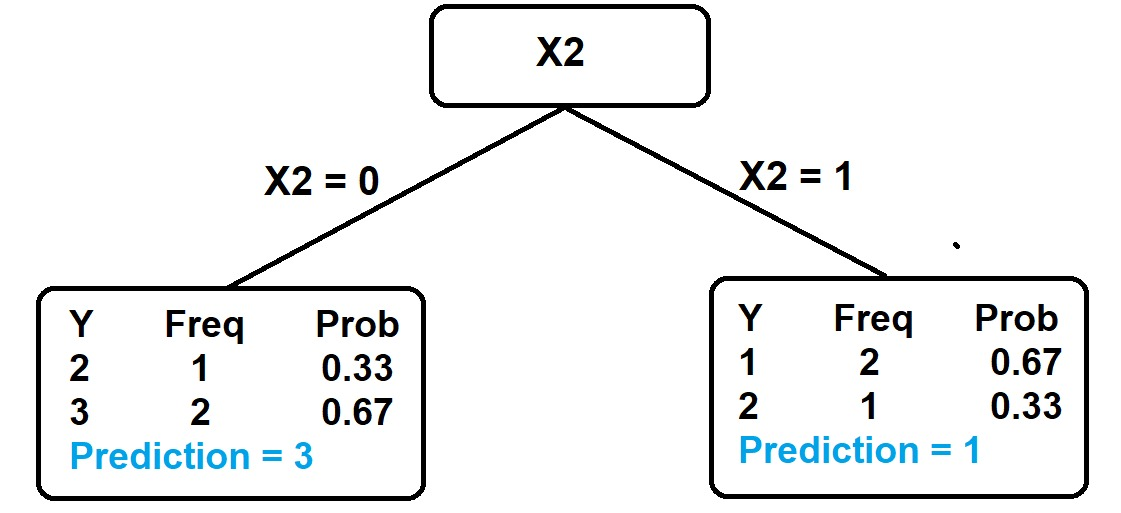
\includegraphics[width=\textwidth]{tree_image.jpeg} % Adjust 'width' based on your requirements
  \caption{Decision tree using X2 for splitting at root} % Adds a caption below the image
  \label{fig:your_label} % Label for referencing the image later
\end{figure}


\subsection*{\underline{Part (3)}:}
Conducting classification for the test example $X_1 = 0$ and $X_2 = 1$.\\
Using our decision tree above, we see that we have to check $X_2$ at root node to decide which side to go.\\
Since $X_2 = 1$, we go to the right side and reach the node which is leaf, where the prediction value is $Y = 1$ based on it's probability.\\
So, for test example $X_1 = 0$ and $X_2 = 1$, we classify $Y = 1$.

\section*{\underline{Problem 2: Entropy}}

\subsection*{\underline{Part (1)}:}

\subsection*{\underline{Part (2)}:}

\subsection*{\underline{Part (3)}:}

\end{document}